\begin{enumerate}
	\item Write the quadratic equation in $x$ whose roots are $2$ and $-5$.
		\item If $\alpha$ and $\beta$ are zeros of the quadratic polynomial $f(x) = x^2 - x - 4$, find the value of $\frac{1}{\alpha} + \frac{1}{\beta} - {\alpha \beta}$.
		\item If one zero of the quadratic polynomial $x^{2} + 3x + k$ is $2$, then find the value of $k$.
		\item If $3\sin A = 1$, then find the value of $\sec A$.
		\item Show that: $\frac{1 + \cot^2{\theta}}{1 + \tan^2{\theta}} = \cot^2{\theta}$.
\item Simplify :$${\csc^{2}{60\degree} \sin^{2}{30\degree} - \sec^{2}{60\degree}}$$
	\item If $\tan{\theta} + \cot{\theta}$ = $\frac{4 \sqrt{3}}{3}$, then find the value of $\tan^{2}{\theta} + \cot^{2}{\theta}$. 
	\item Divide the polynomial $f(x) = 5x^{3} + 10x^{2} - 30{x} - 15$ by the polynomial $g(x) = x^{2} + 1 + x$ and hence, find the quotient and the remainder.
		\item Prove:$$\frac{1}{(\cot A)(\sec A) - \cot A} - \csc A = \csc A - \frac{1}{(\cot A)(\sec A) + \cot A}$$
		\item Prove:$$\sin^{6} A + 3\sin^{2} A \cos^{2} A = 1 - \cos^{6}  A$$
		\item One of the root of the quadratic equation $2x^{2} - 8x - k = 0$ is $\frac{5}{2}$. Find the value of $k$, Also find the root.
		\item Using quadratic formula, solve the following equation for x:$$abx^{2} + (b^{2} - ac)x - bc = 0$$.
	\item With vertices A,B and C of a triangle ABC as centers, arcs are drawn with radii $2$ cm each as/ shown in the figure. If AB = $6$ cm, BC = $8$ cm and AC = $10$ cm, find the area of the shaded region.	  	
	\begin{figure}[h]
	      			\centering
	      			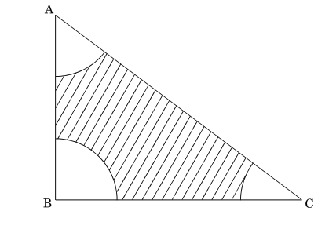
\includegraphics[width=\columnwidth]{figs/triashaded.jpg}
				\caption{}
				\label{fig:xxxx}
      \end{figure}
	\item Water is being pumped out through a circular pipe whose internal diameter is $8$ cm. If the rate of flow of water is $80$ cm/s, then how many liters of water is being pumped out through this pipe in one hour ?
		\item A man on the top of a vertical tower observes a car moving at a uniform speed coming directly towards it. If it takes $18$ minutes for the angle of depression to change from $30\degree$ to $60\degree$, how soon after this will the car reach the tower ?

		\item A girl on a ship standing on a wooden platform, which is $50$ m above water level, observes the angle of elevation of a top of a hill as $30\degree$ and the angle of depression of the base of the hill as $60\degree$. Calculate the distance of the hill from the platform and the height of the hill.
\end{enumerate}
